\documentclass[12pt,a4paper]{article}
\usepackage[a4paper, left=2cm, right=2cm, top=2cm, bottom=2cm]{geometry} 
\usepackage[final]{graphicx}
\usepackage{subcaption}
\usepackage[export]{adjustbox}
\usepackage{amsmath,float,bm}
\usepackage[affil-it]{authblk}
\usepackage{titlesec,wrapfig,amssymb}
\usepackage{empheq}
\usepackage{amsthm}
\usepackage[T1]{fontenc}
\usepackage[polish]{babel}
\usepackage[utf8]{inputenc}
\usepackage{graphicx}
\usepackage{hyperref}
\graphicspath{ {photos/}}


\begin{document}
\newtheorem{fakt}{Fakt}
\begin{flushleft}
Jakub Swistak\\
Poland \\
kontakt@jakub0301.net\\
Stanford SUMAC \\

\end{flushleft}\


\section*{}



\begin{proof}[Solution to task number 1]

$x^2-y^2=(x+y)(x-y)$\\
Firstly let's factorize $2019=3 \cdot 673$. We can see that 3 and 673 are prime numbers. We can also notice that $x+y>x-y$ because $x$ and $y$ are positive. Hence,
$$\left\{\begin{array}{rcl}
x+y=673\\
x-y=3\\
\end{array} \right.$$

$$\left\{\begin{array}{rcl}
2x=673\\
x-y=3\\
\end{array} \right.$$

$$\left\{\begin{array}{rcl}
x=338\\
y=335\\
\end{array} \right.$$\\
or 
$$\left\{\begin{array}{rcl}
x+y=2019\\
x-y=1\\
\end{array} \right.$$

$$\left\{\begin{array}{rcl}
2x=2020\\
x-y=1\\
\end{array} \right.$$

$$\left\{\begin{array}{rcl}
x=1010\\
y=1009\\
\end{array} \right.$$

$x^3-y^3=(x-y)(x^2+xy+y^2)$\\

 Then simply we can notice that $x-y<x^2+xy+y^2$

$$\left\{\begin{array}{rcl}
x-y=3\\
x^2+y^2+xy=673\\
\end{array} \right.$$

$$\left\{\begin{array}{rcl}
x=3+y\\
(3+y)^2+y^2+(3+y)y=673\\
\end{array} \right.$$

$0=(3+y)^2+y^2+(3+y)y-673=2y^2+5y-667$\\
 $\Delta =5361 $ and $ \sqrt[2]{5361} \notin \mathbb{N}$ $\Rightarrow$ there are no solutions.
Or 
$$\left\{\begin{array}{rcl}
x-y=1\\
x^2+y^2+xy=2019\\
\end{array} \right.$$ 

$$\left\{\begin{array}{rcl}
x=1+y\\
(1+y)^2+y^2+(1+y)y=2019\\
\end{array} \right.$$ 

$$\left\{\begin{array}{rcl}
x=1+y\\
3y^2+3y-2018=0\\
\end{array} \right.$$ 
$\Delta=24225$ and $ \sqrt[2]{24225} \notin \mathbb{N}$ $\Rightarrow$ there are no solutions.
 
\end{proof}
\vspace{1cm}
\begin{proof}[Solution to task number 2]

Let's suppose $p(\sqrt[]{7}-\sqrt[]{3})=0$ and $\deg(p)=4$ $\Rightarrow p(\sqrt[]{7}-\sqrt[]{3})= a_0+a_1(\sqrt{7}-\sqrt{3})+a_2(\sqrt{7}-\sqrt{3})^2+a_3(\sqrt{7}-\sqrt{3})^3+a_4(\sqrt{7}-\sqrt{3})^4=0$\\
Then after expending every bracket we obtain:

\begin{align}
\sqrt{7}(a_1+16a_3)+\sqrt{3}(-a_1-24a_3)+\sqrt{21}(-2a_2-40a_4)+184a_4+10a_2+a_0=0\label{p2eq:1}
\end{align}

Observe that equation \eqref{p2eq:1} holds if

$$\left\{\begin{array}{rcl}
a_1+16a_3=0\\
a_1+24a_3=0\\
a_2+20a_4=0\\
a_0+10a_2+184a_4=0\\
\end{array} \right.$$

$$\left\{\begin{array}{rcl}
a_3=0\\
a_1=0\\
a_2=-20a_4\\
a_0+10a_2+184a_4=0\\
\end{array} \right.$$

$$\left\{\begin{array}{rcl}
a_3=0\\
a_1=0\\
a_0=16a_4\\
a_2=-20a_4\\
\end{array} \right.$$

Let $a_4=1  \Rightarrow a_0=16$ and $a_2=-20 \Rightarrow p(x)=x^4-20x^2+4$ 

\end{proof}
\vspace{1cm}
\begin{proof}[Solution to task number 3] Firstly let's replace black element with $6$.

\[
 \begin{matrix}
  1 & 2 & 3 \\
  4 & 5 & 6 \\
 \end{matrix}
\]
Let's define $\pi(x)$ gives us position of the element, then for example $\pi(4)=4$. Let's notice that first matrix is identity. Let's also notice that we have to "go" with $6$ to element and then "go back", then we will make $2n$ moves. \\
$sgn(\pi_1 \circ\ pi_2)=sgn(\pi_1)*sgn(\pi_2)$\\
Then for first matrix $sgn(t_1\circ...\circ t_{2n})=1$\\


\[
 \begin{matrix}
  2 & 1 & 3 \\
  4 & 5 & 6 \\
 \end{matrix}
\]
For second matrix $sgn(t_1\circ...\circ t_{2n+1})=-1$\\
which gives us a contradiction
\end{proof}
\vspace{1cm}
\begin{proof}[Solution to task number 4]
\
\\

a) Let's divide the triangle to $4$ congruent equilateral triangles with side-length $0.5$ cm each (see the picture below). If we select $5$ points then since there are only $4$ triangles, thus one of the triangles will contain two points. The distance between these two points is not greater then $0.5$ cm which is the diameter of the triangle.

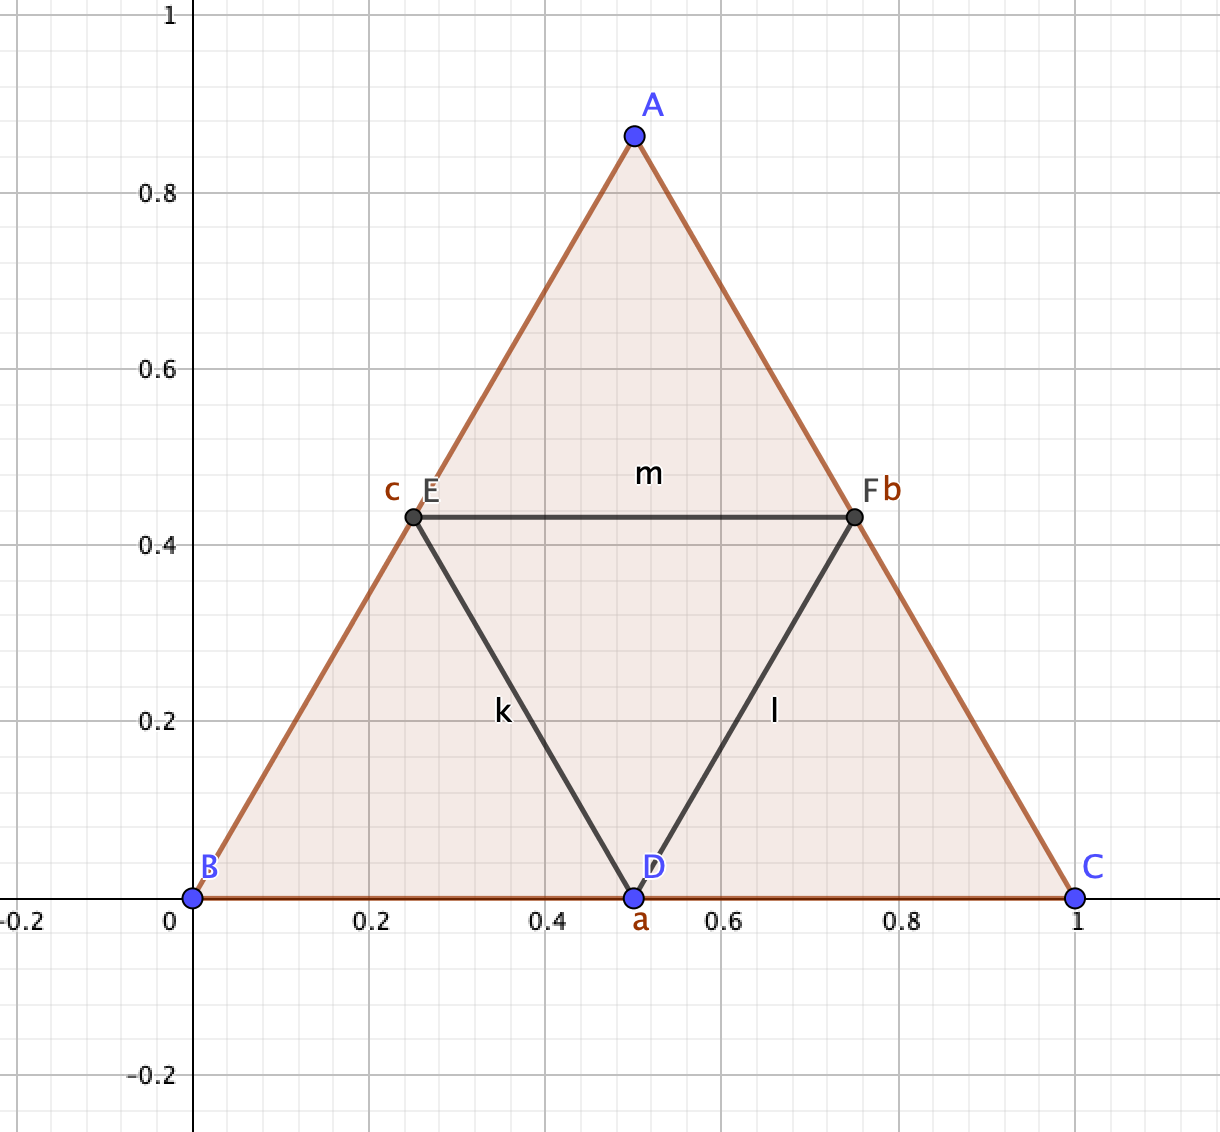
\includegraphics[scale=0.4]{triangle}

b) Let's take points A,B,C,D,E and F from the picture. They are the vertices of the 0.5 cm triangles and the picture shows that the distance between each pair will be exactly $0.5$ cm.

c) Let's divide triangle as on the picture below to $3$ congruent equilateral triangles with side-length $0.45$ cm and to $3$ congruent quadrangles. With the longest diameter equal $0.48$ cm $ \Rightarrow$ It will work for $7$ points. $\Rightarrow$ It will work for $8$ points.\\
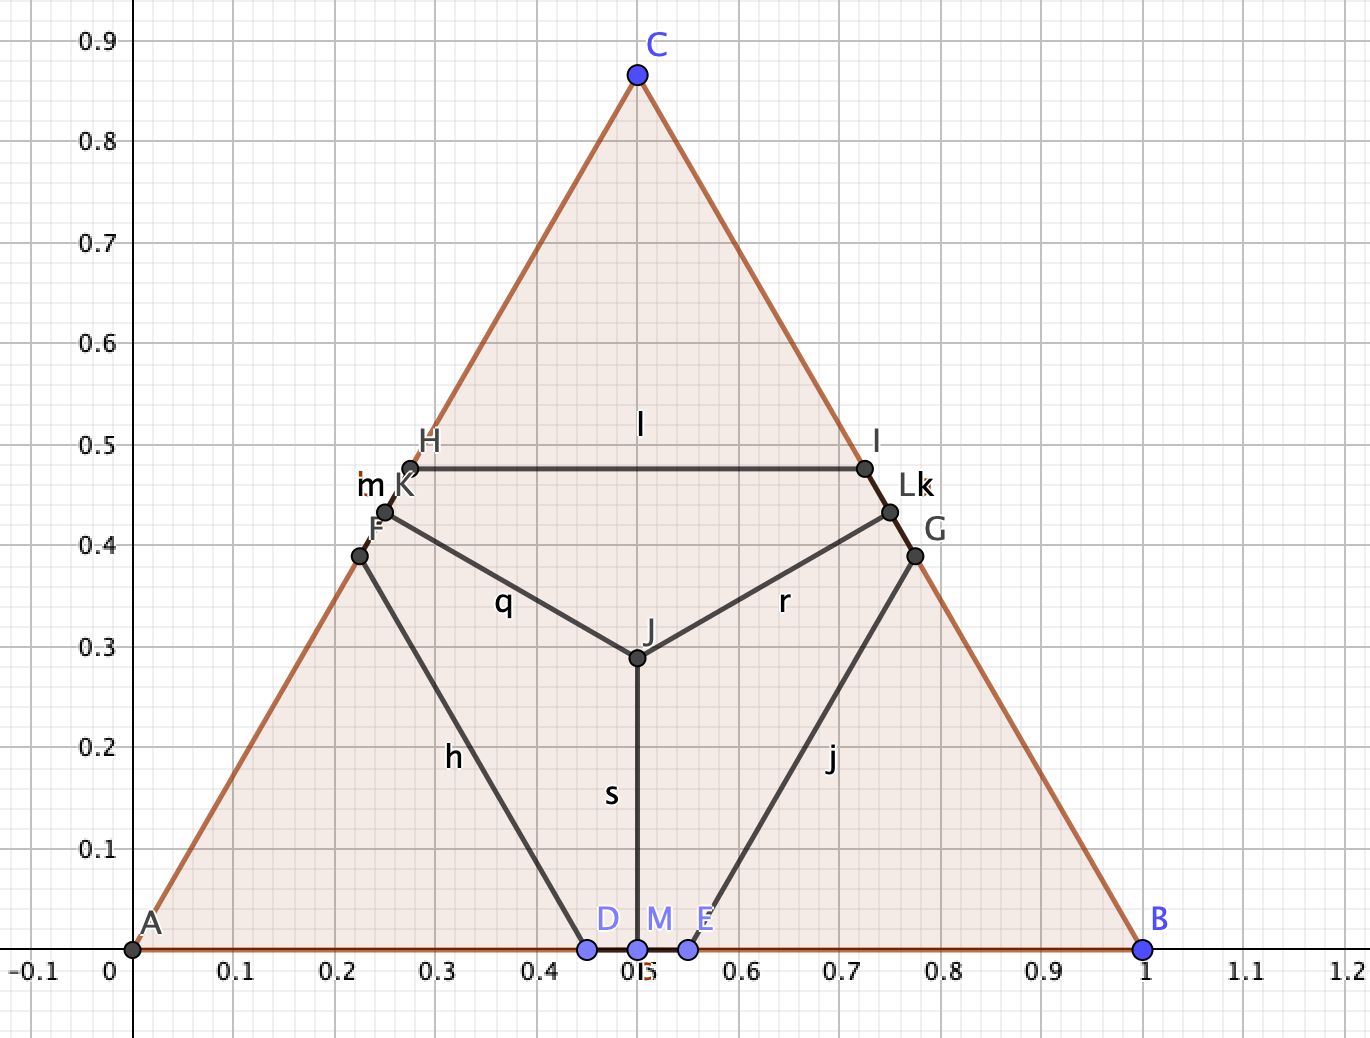
\includegraphics[scale=0.4]{p2}
\end{proof}
\vspace{1cm}


\begin{proof}[Solution to task number 5]
\
\\

a) The number of islands equals to the number of $0-1$ sequences of length $n$ which is $2^n$. For any island we have $n$ islands which differ on a one bit, each island is connected with remaining islands with $n$ routes (cause it can be diffrent in $n$ positions), then $\frac{2^n*n}{2}$ 

[Here I was looking for some more ideas (to solve for $n=5$ and $n=6$) and found some articles about Hypercube and Hamming distance]
Let K be the gratest subset of vertices of Hypercube Q=(V,E), such that for any vertices $v_1,v_2$ in K occurs $dist(v_1,v_2)\geq3$ (Hamming distance).
\\
$|K|\leq \frac{2^n}{n+1}$ (because every vertex from $K$ will remove himself and $n$ connected with direct edge)
$|K|*(deg(v)+1)\leq |V|$\\

n=3\\

$K=\{000,111\}, |K|=2$ (cube)\\


n=4\\
without loss of generality $K$ contain $\{0000\}$, so
$\{v: dist(v,0000)\geq 3\}=\{1111,1110,1101,1011,0111\}$
Let's notice that  in the set above distance between every pair of points is $\leq2$, so we can pick only two points $\Rightarrow K=\{0000,1111\}, |K|=2$

n=5\\
We are using very similar idea like in $n=4$
without loss of generality $K$ contain $\{00000\}$, so $\{v: dist(v,00000)\geq 3\}=\{binary\ strings\ with\ 3\ or\ 4\  ones\}$
If we add $\{11111\}$, we will not be able to add because $\{v: dist(v,11111)\geq 3\}=\{strings\ with\ 3,\ 4\ or\ 5\ zeros\}$ therefore ${v: dist(v,11111)\geq 3} \cap {v: dist(v,00000)\geq 3}=\emptyset$
\\
WLG-without loss of generality\\
Now let's consider when we will add string with $4$ ones WLG  it will be $11110 \Rightarrow 
\{v: dist(v,00000)\geq 3$ and  $dist(v,11110)\geq 3\}=$\\ $\{00111,10011,11001,01011,10101,01101\}$
Distance between every two vertices listed above is $2$ or $4$ and it's impossible to pick $3$, so as to distance between will be $4$.$\Rightarrow$ we can add only $2$ more vertices $\Rightarrow K=\{00000,11110,00111,11001\}$  \\
Case when $K$ doesn't contain $4$ ones will  be similar, but $|K|$ will be smaller

n=3

M={000,111} |M|=2

n=4

$|M|\geq\frac{16}{5}$, therefore $|M|\geq 4$
Easily we can check, that  $\{0000,1001,1110,0111\}$  $|M|=4$

n=5

$|M|\geq\frac{32}{6}$, therefore $|M|\geq 6$
The greatest set which I have found  is \\
$\{00000,11110,00111,11001,10011,01011,01100,10100\}$.
\end{proof}
\vspace{1cm}
\begin{proof}[Solution to task number 6]
\
\\
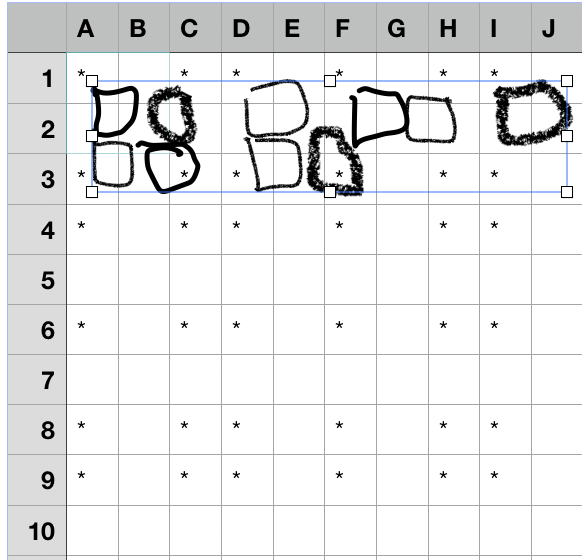
\includegraphics[scale=0.7]{kon1}\\
a) Let's consider the following construction(image above) by star denote area covered by only one $2$x$2$ card and by (1A,2B) denote $2$x$2$ card covering filed from A1 to B2.\\
 There are 36 stars and every block are covering exactly one star(blocks on\\ (A1,B2),(B1,C2),(D1,E2),...,(2A,3B),...(9I,10J). (there are some marked on the picture)
 
 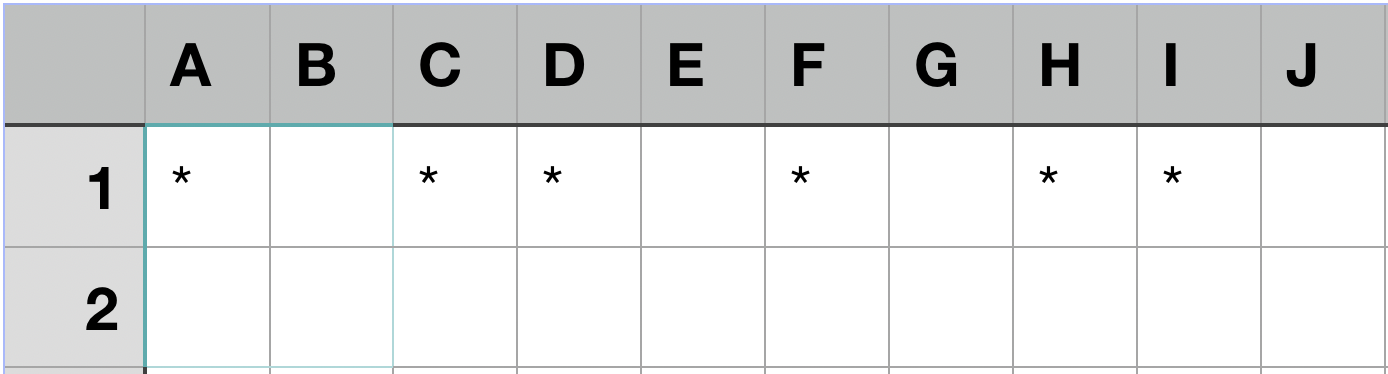
\includegraphics[scale=0.4]{ko}\\
 Let's also notice that this construction will generate the greatest score for non-redundant to prove let's consider $2$x$10$ table and construct greedily, 
then the maximum score which will avoid redundant cards. We can also use the same way to table $10$x$2$ and $"$connect both ideas$"$, which will give construction mentioned earlier.
 It also proves that every covering with 55 cards is redundant.
\end{proof}
\end{document}
